\documentclass[12pt]{report}
\usepackage[pdftex]{graphicx}
\author{James Clements}
\date{Fall 2012}
\title{ME 351A: Inviscid Fluid Mechanics Notes}
\usepackage{textgreek}
\usepackage{fullpage}
\begin{document}
\maketitle
\tableofcontents
\chapter{What is a fluid? - 9/25/2012}
\begin{itemize}
\item Commonsense definition: fluids "fill their container", fluids "takes shape of container
\item Studying fluid mechanics requires more mathematical precision. 
\end{itemize}
\section{Mathematically precise definition of fluid}
(1) A fluid is a substance that deforms$^*$ continuously under the action of any shear$^*$ stress.

We will use continuum assumption to describe fluid flows. Namely, fluid/flow properties are continous and can be defined pointwise in space.

\begin{itemize}
\item[Consider:] A microscopic view of actual fluids
\begin{figure}[h]
\centering
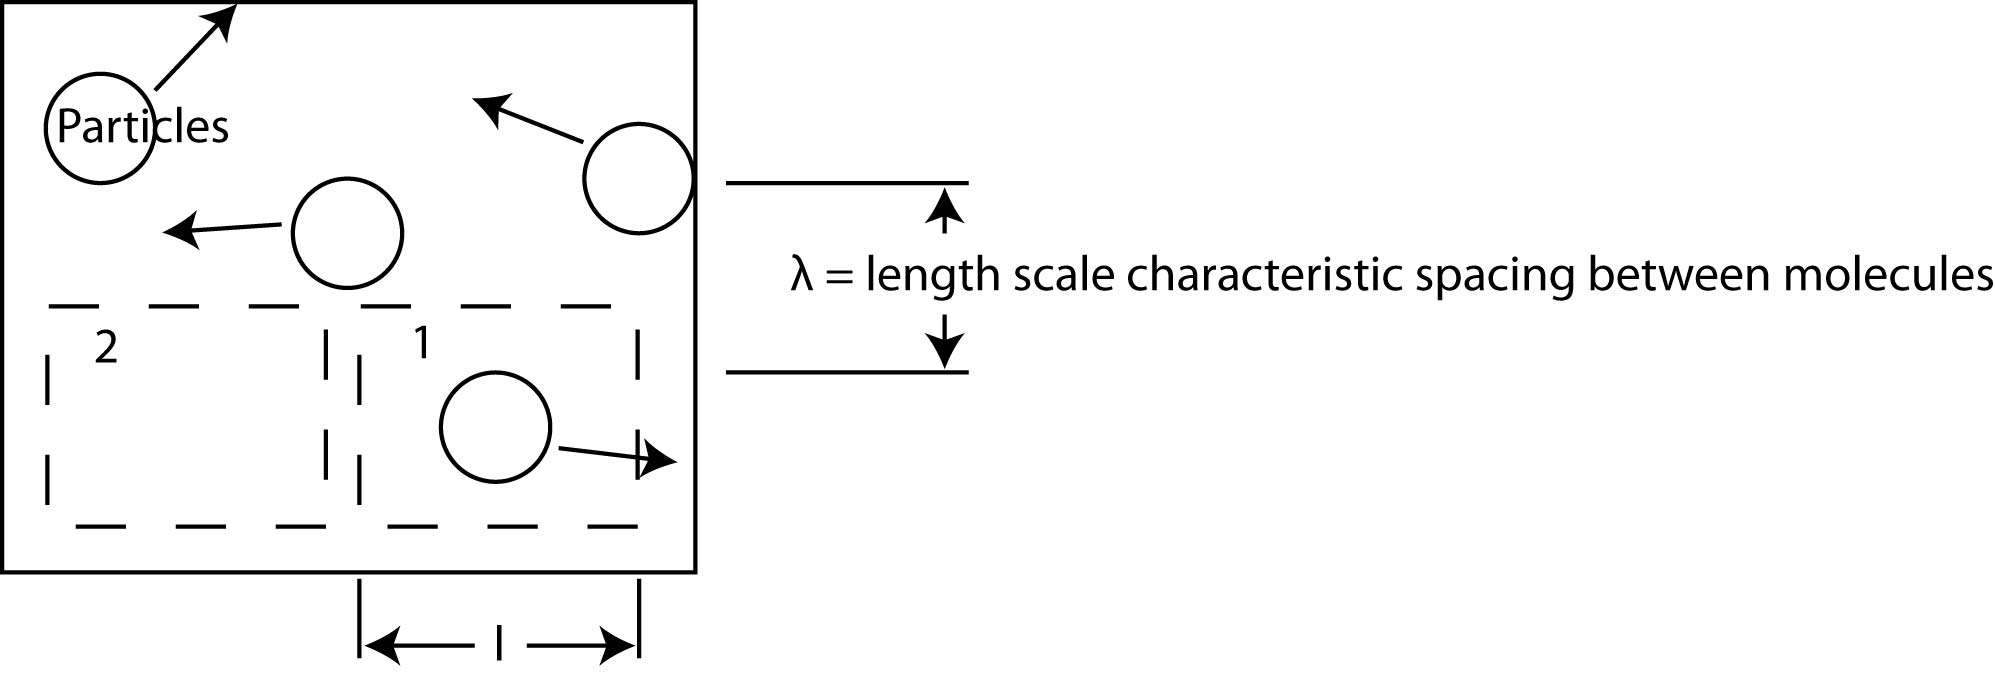
\includegraphics[width=100mm]{MicroscopicFluidExampleME351A.jpg}
\end{figure}
\item Individual particles undergo random motion in a fluid
\item[Suppose] You want to quantify the fluid density, \textrho : $\rho(\bar{x},t) $ which is a function of space and time.

If I use sampling windows spanning lxl:
\item $\rho \neq 0 $ in window 1
\item $\rho = 0$ in window 2
\item[Result: ] To study fluids at the macro level, assume that sampling windows span size l such that:
\[\lambda<<l<<\eta\]
where $\eta$ represents the smallest important scale of the flow system. This will keep my system continuous.
\item Note that $\eta$ is set by flow geometry
\item $\eta_{Gas}$ is between $10^{-7}$ and $10^{-8}$ meters

\item We need a $\lambda<<l$ so properties vary continuously
\item $l<<\eta$ is sued so we can discriminate variations in properties.

\item[In practice: ] do not need to actually define l for most engineering problems. Usually can be confident that such a scale exists. 

\item[\textbf{!Warning}] Might not be able to apply continuum assumption under the following cases:
\item Microfluidics can be problematic if $\eta$ is very small
\item Rarified systems (ie: in space), intermolecualar spacing, $\lambda$, might get very large. This can be a problem too.
\item Study of fluid at molecular scale is field on its own called Kinetic Theory or Physical Fluid Dynamics

\end{itemize}
\section{Fluid Properties}
\begin{itemize}
\item[Scalars:]
\item Zero order tensor
\item no directional information
\item time, t; pressure, p; density, $\rho$; kinematic viscosity $\nu$
\end{itemize}


\end{document}